
%
\section{Introduction} % (fold)
\label{sec:tcl_introduction}
%
Feature extraction is one of the most successful standard approaches in
Scientific Visualization.
%
Features describe important and relevant properties of a field.
%
Their extraction and representation promises an effective visualization of even
complex data sets.
%
For scalar and vector fields, a variety of features have been proposed.
%
The most prominent ones for vector fields are topological features and vortices.
%
For the extraction of vortex core lines, a standard approach is the one by
Sujudi and Haimes \cite{Sujudi1995}.
%
It finds all locations in a piecewise linear vector field where the Jacobian has
complex eigenvalues and the streamlines are parallel to its single real
eigenvector.
%
It is known that these lines can be characterized in terms of the \ac{PV}
operator \cite{Peikert1999}, which has also been used to extract ridge and
valley lines, and separation and attachment lines.
%
Locations where the flow is parallel to an eigenvector of a Jacobian with three
real eigenvalues also form stable lines.
%
These hyperbolic trajectories are the centers of simultaneous converging and
diverging behavior of the vector field and can be used to extract Lagrangian
coherent structures~\cite{Machado2013,Machado2016}.
%
Roth and Peikert~\cite{Roth1998} showed that vortex core lines can equivalently
be described as locations where the curvature of streamlines locally vanishes.
%

%
\begin{figure}
    \centering
    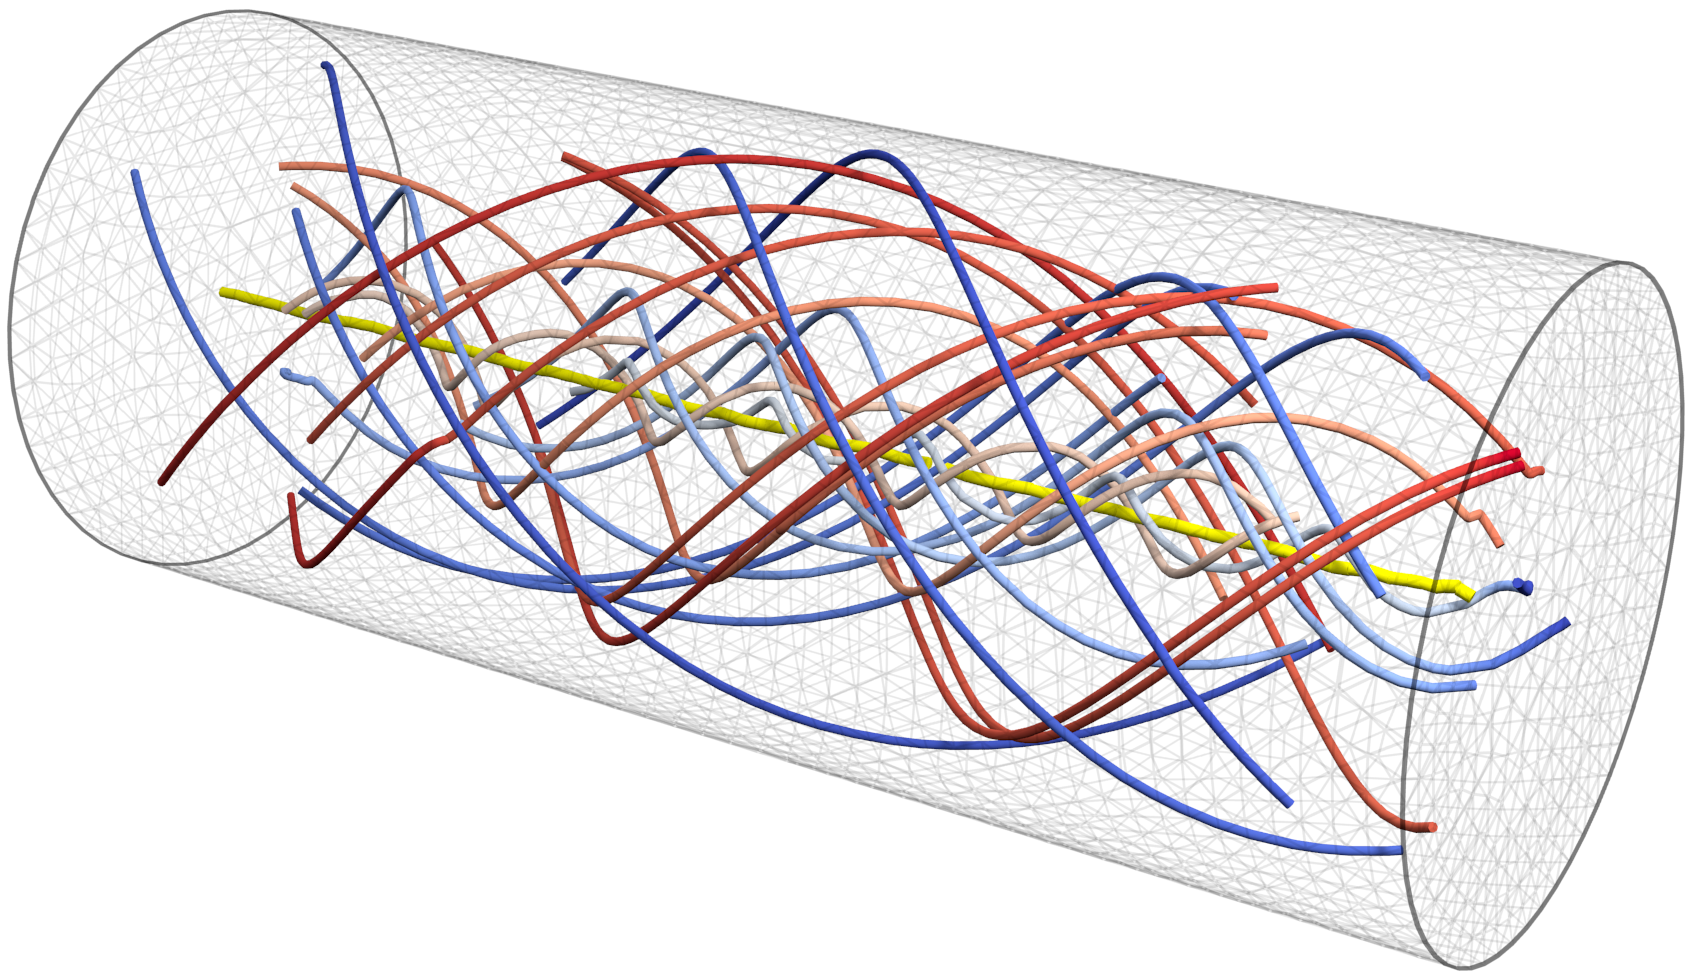
\includegraphics[width=\columnwidth]{figures/torque_tube_lines.png}
    \caption{Eigenvector trajectories in a stress tensor field induced by
             applying a torque to a cylindrical shaft. Trajectories of both
             major (blue) and minor (red) eigenvectors show a swirling behavior
             around a common core line (yellow).}
    \label{fig:tube_lines}
\end{figure}
%
In this work, we examine three-dimensional, second-order tensor fields, \ie,
functions that map a matrix in $\RRSet^{3 \times 3}$ to each location in a
three-dimensional domain.
%
Tensor fields arise from a variety of applications in physics.
%
Examples are stress and strain-, deformation-, and diffusion
tensors.
%
In second-order tensor fields, the analog of stream lines are eigenvector
trajectories.
%
These are lines that are tangential to an eigenvector of the tensor field
everywhere along their path.
%
Eigenvector trajectories can show a behavior similar to vortices in vector
fields.
%
For example, solid objects subject to a torque show swirling eigenvector
trajectories of the stress tensor field (see \autoref{fig:tube_lines}).
%
A number of topological visualization methods have been proposed for
second-order tensor fields.
%
However, there are no approaches to extract core lines of tensor fields similar
to Sujudi/Haimes and the \ac{PV} operator for vector fields.
%
Such an approach would be a valuable tool for quickly identifying regions with
swirling behavior of eigenvector trajectories, such as induced by torque, that
would otherwise be tedious to find.
%
In this paper, we introduce the concept of {\em tensor core lines} as all
locations in the \ac{3D} domain of a tensor field where at least one eigenvector
trajectory has a vanishing curvature.
%
Considering the observation made by Roth and Peikert~\cite{Roth1998}, this is
the direct extension of Sujudi/Haimes to tensor fields.
%
In particular, we make the following contributions:
%
\begin{itemize}
    \item  We give a rigorous definition of tensor core lines and show that the
    definition gives indeed structurally stable line structures.
    %
    \item We provide a numerical algorithm for the extraction of tensor core
    lines in piecewise linear tensor fields.
    %
    \item We introduce a filter criterion based on numerical stability to
    separate significant and insignificant tensor core lines.
    %
    \item We show tensor core lines in mechanical stress tensor fields,
    interpret them and compare them with degenerate lines where two eigenvalues
    are equal.
\end{itemize}
%

%
\subsection*{Relation of Tensor Core Lines to the Parallel Vectors Operator}
%
At first glance, tensor core lines seem to be a straightforward extension of the
classical \ac{PV} operator:
%
given a tensor field, we consider all eigenvector fields as vector fields
and apply the \ac{PV} operator to them.
%
Such a naive approach cannot give well-defined and stable results for the
following reasons:
%
\begin{itemize}
    \item
    Undefined length and orientation of eigenvectors:\\
    %
    An eigenvector of a matrix is in fact not a vector but a linear subspace.
    %
    To express the field of eigenvectors as a vector field, heuristic
    assumptions about the length and orientation of the vectors are necessary.
    %
    Applying such assumptions globally can not always give results that are
    free of discontinuities.
    %
    \item
    Existence of multiple eigenvectors:\\
    %
    Regions with three real eigenvectors require a decision on which of them to
    use for the \ac{PV} operator -- a decision that is particularly non-unique in
    near-isotropic regions (i.e., where the difference between two real
    eigenvalues is small).
    %
    \item
    Discontinuities in eigenvectors:\\
    %
    A small change of a tensor does not necessarily result in a small change of
    the eigenvectors.
    %
    In fact, in near-isotropic regions, a small change of the tensor may result
    in a very large change of the eigenvector.
    %
    Moreover, in regions of transition between real and imaginary eigenvalues
    (i.e., in neighborhoods containing both tensors with all real eigenvalues
    and tensors with complex eigenvalues), a small change of the tensor can
    result in a sudden appearance or disappearance of real eigenvectors.
    %
\end{itemize}
%
Some of the problems mentioned above could be tackled by local heuristics (for
instance, the orientations of the eigenvectors in a local neighborhood could be
chosen as consistent as possible).
%
However, especially the last point shows that eigenvectors show a fundamentally
different behavior than normal vector fields for which the \ac{PV} operator is
designed.
%
New algorithms for the extraction of tensor core lines are therefore necessary.
%
% section introduction (end)